\documentclass[10pt]{article}
\usepackage{amsmath,listings,graphicx,caption,subfig,float,subfig}
\usepackage[margin=0.5in]{geometry}

\begin{document}
\noindent
Robert Werthman\\
CSCI 5622\\
Homework 4: Boosting\\

\section*{Question 2}
The \textbf{decision tree boosting classifier} was trained on the training set given in boosting python file.  The classifier was then tested with the testing 
set given in the boosting python file.  I looked at the accuracy of the set 
of the number of learners \{1, 10, 50, 100, 300\} and the set of depths \{1, 2, 3, 4\}.  
For each depth I calculated the accuracy for each different number 
of learners.  Accuracy is the number of correctly predicted samples from 
the testing set divided by the total number of samples in the testing set.  Error is 1 minus this accuracy.\\
\\
Based on the graph of the accuracy of the decision tree boosting with the training set vs the accuracy of the decision tree boosting with the test set, I noticed the following things:
\begin{enumerate}
  \item It appears that no matter what depth the decision tree 
  weak learners are initialized to, the more weak learners you have the more 
  accurate the classifier is.
  \item The greater the depth the decision tree weak learners are initialized to, the higher the initial and final accuracies are of the classifier.
  \item The accuracy of predictions of the decision tree boosting is greater with the training set than with the test set.  It is not significantly greater, but it is possible this is due to overfitting.  The classifier does not do as well on the test set as it does on the training set.
\end{enumerate}

\section*{Question 3}
The \textbf{multinomial naive bayes boosting classifer} was trained on 
the same training set the \textbf{decision tree boosting classifier} was trained on.  
The classifer was then tested on the same test set as the \textbf{decision tree boosting classifier}.  I looked at the accuracy of the classifier at each value in the set of the number of learners \{1, 10, 50, 100, 300\}.\\
\\
As can be seen in the graph of the \textbf{multinomial naive bayes boosting classifer}, it had the worst final and initial accuracies when compared to the \textbf{decision tree boosting classifier} at all four depths.  It appears the \textbf{decision tree boosting classifier} is better as a weak learner for boosting than the \textbf{multinomial naive bayes boosting classifer}.

\begin{figure}[H]
\centering
  \subfloat[Accuracy of decision tree test set]{
  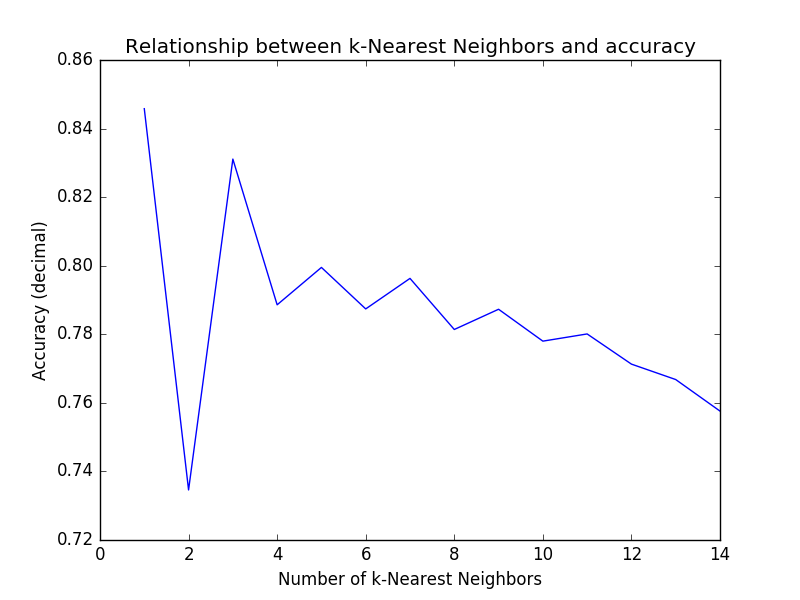
\includegraphics[scale=.32]{q2.png}
  }
  \subfloat[Accuracy of decision tree training set]{
  \includegraphics[scale=.32]{q2_train_accuracy.png}
  }
  \subfloat[Accuracy of multinomial naive bayes test set]{
  \includegraphics[scale=.32]{q3.png}
  }
 \caption{Decision Tree and Multinomial Naive Bayes Boosting}
\end{figure}

\end{document}